
\documentclass[12pt]{report}
\usepackage[Glenn]{fncychap}
\usepackage[T1]{fontenc}
\usepackage[francais]{babel}
%\usepackage{fontspec}
\usepackage{wrapfig}
\usepackage{graphicx}
\usepackage{soul}
\usepackage[colorlinks=true, linkcolor=black, urlcolor=black, citecolor=black]{hyperref}
% \usepackage[hyphens, spaces, obeyspaces]{url}
\usepackage[a4paper, width=150mm, top=25mm, bottom=25mm]{geometry}
\usepackage{parskip}
\usepackage{enumitem}
\usepackage{titlesec}
\usepackage{listings}
\usepackage{float}
\usepackage[final]{pdfpages}
\usepackage{xcolor}
\usepackage{tocbibind}
\usepackage{tocloft}
\usepackage[utf8]{inputenc}
\usepackage{xpatch}
\usepackage{amsmath}
\usepackage{amsthm}
\usepackage{amsfonts}
\usepackage{graphics}
\usepackage{color}
% \usepackage[grey,utopia]{quotchap}
\usepackage{moreverb}
\usepackage{xcolor}
\usepackage{framed}
\usepackage{arabluatex}
\usepackage[algo2e, french, onelanguage, ruled]{algorithm2e}
\setlist[itemize]{label=\textbullet}
\usepackage{fancyhdr}
\pagestyle{fancy}   
\fancyhead{}
\fancyhead[C]{\leftmark}
\renewcommand{\headrulewidth}{0.4pt}
\renewcommand{\footrulewidth}{0.4pt}
\usepackage{xcolor}
\definecolor{light-gray}{gray}{0.90}
\newcommand{\code}[1]{\colorbox{light-gray}{\texttt{#1}}}
\usepackage{listings}
\usepackage{multirow}

\usepackage{array}
\newcolumntype{L}[1]{>{\raggedright\let\newline\\\arraybackslash\hspace{0pt}}m{#1}}
\newcolumntype{C}[1]{>{\centering\let\newline\\\arraybackslash\hspace{0pt}}m{#1}}
\newcolumntype{R}[1]{>{\raggedleft\let\newline\\\arraybackslash\hspace{0pt}}m{#1}}

\lstdefinestyle{code}{
language=python,                   
keywordstyle=\color{blue},      
stringstyle=\color{blue},        
commentstyle=\color{gray},     
basicstyle=\small\ttfamily,           
numbers=left,                   
numberstyle=\normalsize,        
numbersep=7pt,                  
showstringspaces=false,         
breaklines=true,                
frame=leftline,                 
framerule=2pt,
}

\lstdefinestyle{api}{
language=python,                   
keywordstyle=\color{blue},      
stringstyle=\color{blue},        
commentstyle=\color{gray},     
basicstyle=\small\ttfamily,           
% numbers=false,                   
numberstyle=\normalsize,        
numbersep=7pt,                  
showstringspaces=false,         
breaklines=true,                
frame=leftline,                 
framerule=2pt,
}


%~~~BEGIN~~~%
\begin{document}

\newpage
\setlength{\parindent}{0.5cm}

%%% Cover Page %%%
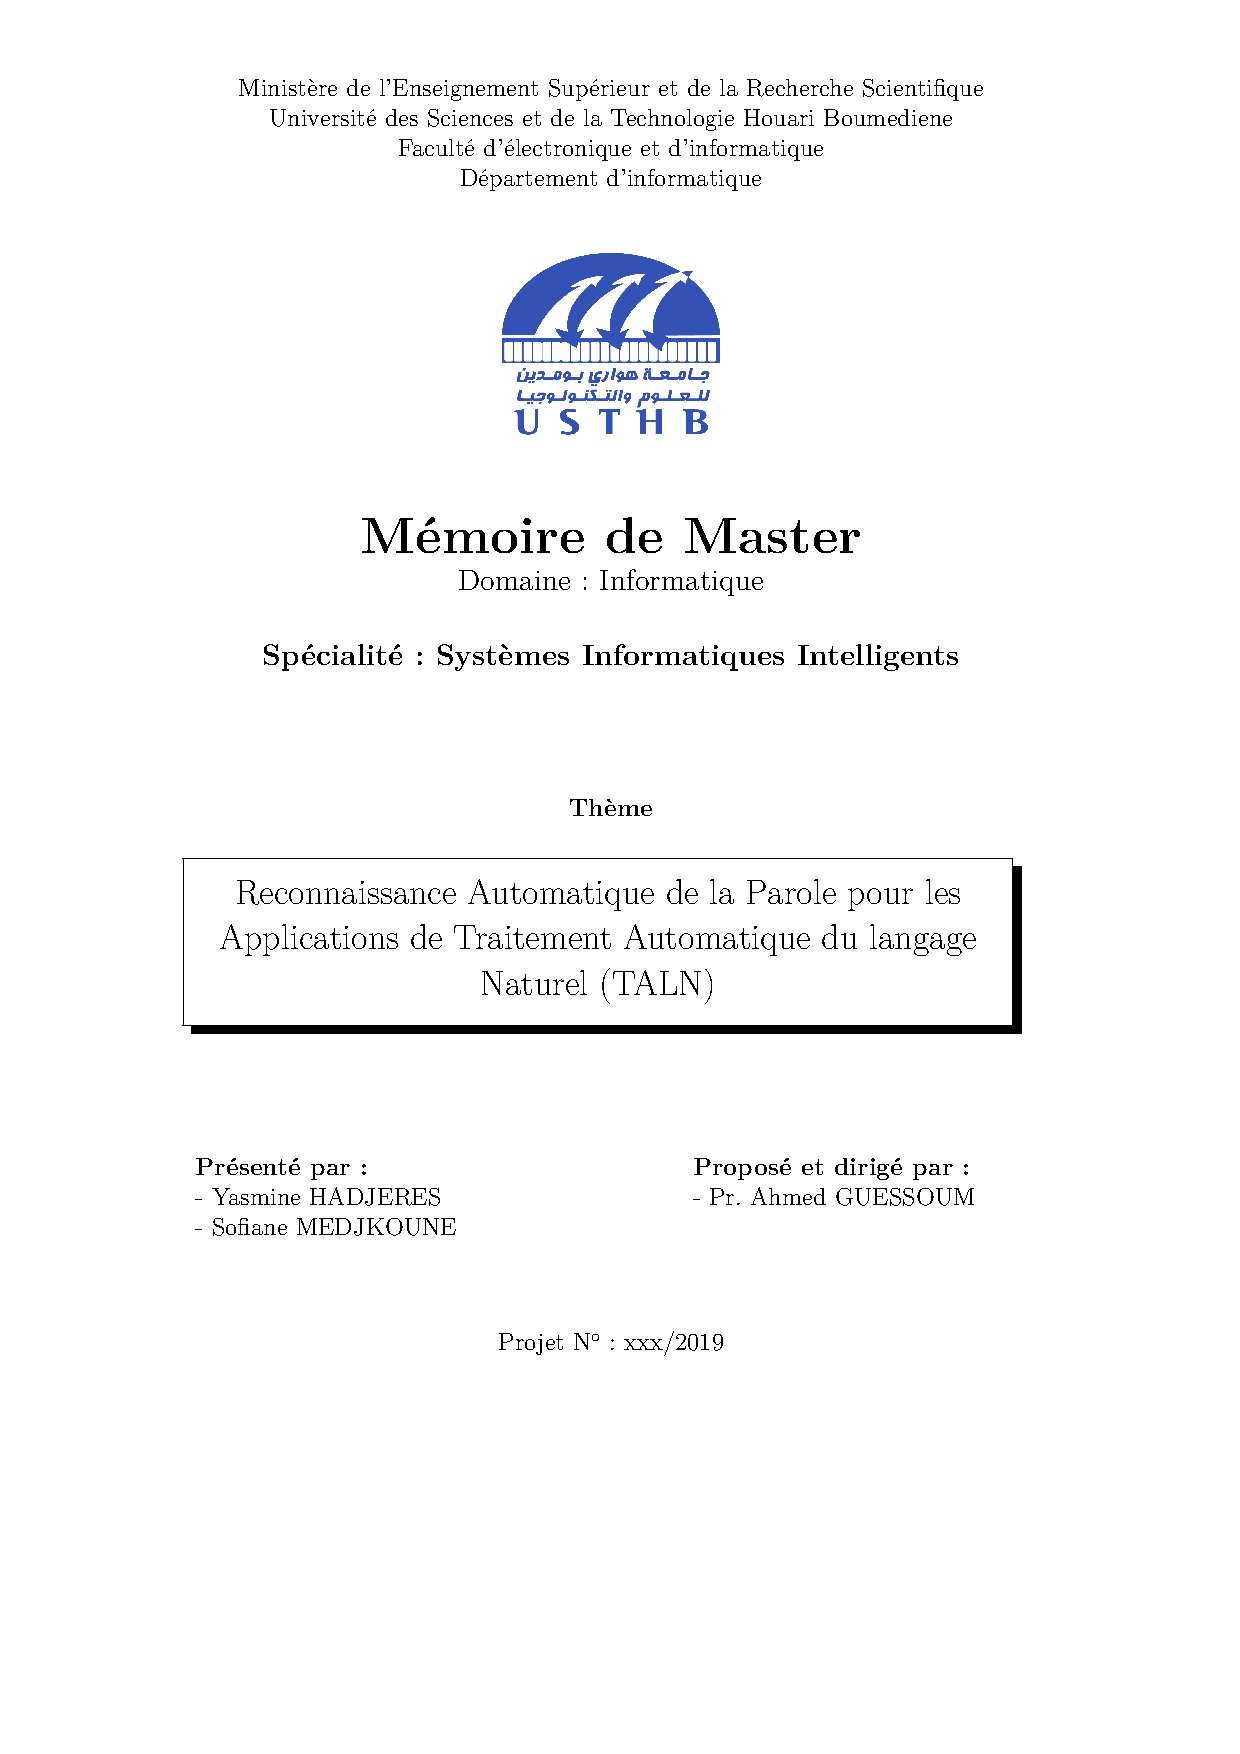
\includepdf[pages=1]{cover.pdf} 

%%% Content tables %%% 
\pagenumbering{gobble}
\renewcommand{\contentsname}{Sommaire}
\tableofcontents
\clearpage

\listoffigures
\clearpage

\listoftables
\clearpage

\listofalgorithmes
\clearpage

%%% NO-plagiat declaration %%%
\newpage    

%%% Chapters %%%
\pagenumbering{arabic} 
\chapter{Automatic Speech Processing (temp title)}
\section{Introduction}
Dans le but de rendre notre interaction avec les outils technologiques plus intuitive, nous nous sommes servi de la voix pour remplacer l'utilisation du clavier.
Pour ce faire, il a fallu développer des systèmes de reconnaissance de la parole. Ces systèmes devaient être capables d'interpréter le langage naturel humain et le transformer en requêtes afin qu'il soit utilisé dans d'autres domaines tel que les systèmes de questions-réponses.

Dans ce chapitre, nous présentons les principes et composants de base des systèmes de reconnaissance de la parole, systèmes de synthèse vocale et des systèmes de questions-réponses.


\section{Reconnaissance de la parole}
\subsection{Définition}
La reconnaissance de la parole, ou speech recognition en anglais, est la capacité d'une machine à comprendre des mots parlés. Un microphone enregistre la voix d'une personne et le matériel convertit le signal d'ondes sonores analogiques en un signal audio numérique. Les données audio sont ensuite traitées par un système, qui retranscrit ces dernières en mots \cite{speechrecdef}.

D'après \cite{speechlangprocessing}, tout bon système de reconnaissance de la parole doit pouvoir reconnaître un vocabulaire étendu (entre 20000 et 60000 mots distincts en moyenne), ne doit pas dépendre de l'orateur et doit traiter un discours continu qui est en accord avec le langage naturel humain.

Ces systèmes reposent sur deux approches :
\begin{itemize}
    \item Architecture basée sur la reconnaissance de phonèmes : qui est considérée comme l'approche classique pour cette tâche de reconnaissance.
    \item Architecture bout à bout (End-To-End en anglais) : qui se base sur les techniques les plus avancées de l'apprentissage artificielle pour des systèmes plus performants mais également plus flexibles.\\
\end{itemize}

La reconnaissance de la parole est classée comme un domaine multidisciplinaire qui se base sur les statistiques, l'apprentissage automatique, la phonétique, la linguistique, le traitement de signal et une profonde compréhension des techniques d'intelligence artificielle.

\subsection{Historique}
La parole est le principal moyen de communication entre les humains. À cet effet, le domaine de la reconnaissance de la parole a attiré beaucoup d'attention au cours des six dernières décennies. Les premières expérimentations virent le jour au cours des années 1950s avec le système “Audrey” en 1952 \cite{audrey} qui reconnaissait des chiffres émis par un unique orateur. En 1962 IBM présente “Shoebox” \cite{ibmshoebox}, un système permettant de reconnaître 16 mots de la langue anglaise. Malgré ces premières avancées, c'est dans les années 1970s que ce domaine décolle réellement avec le système militaire “Harpy” \cite{harpy} qui pouvait reconnaître 1011 mots, ce qui représentait le vocabulaire d'un enfant de 3 ans. Les années 1980s furent marquées par l'utilisation de nouvelles méthodes statistiques pour la prédiction qui, en théorie, permettaient de prédire un nombre illimité de mots. Mais, si ce n'était pas le cas en pratique à cette époque là, ce le fut deux décennies plus tard \cite{speechrechist}. Les systèmes de reconnaissance de la parole n'ont cessé de se perfectionner au cours des années 1990s et 2000s comme le détaille \cite{audreysiri} pour atteindre le statut d'état de l'art dans les années 2010s ce qui correspond à l'utilisation répandue de l'apprentissage automatique ouvrant ainsi la porte à de nouvelles approches que nous découvrons dans la suite de ce document. 

Il est important d'ajouter que ce ne sont pas que les performances de ces systèmes qui ont évolué au fil des décennies mais également les paramètres que nous prenons en compte lors de la reconnaissance de la parole. Alors que ces systèmes ne pouvaient donner de résultats concluants que si le discours était formel et restreint, les requêtes élémentaires et bien définies, l'environnement propre et sans bruit, la prononciation académique et monolingue, nos systèmes sont aujourd'hui capables de faire de la reconnaissance sous tout type de conditions comme le mentionnent \cite{deeplearningapproach} dans la figure \ref{evolotion} ci-dessous. 

\begin{figure}[H]
    \centering
    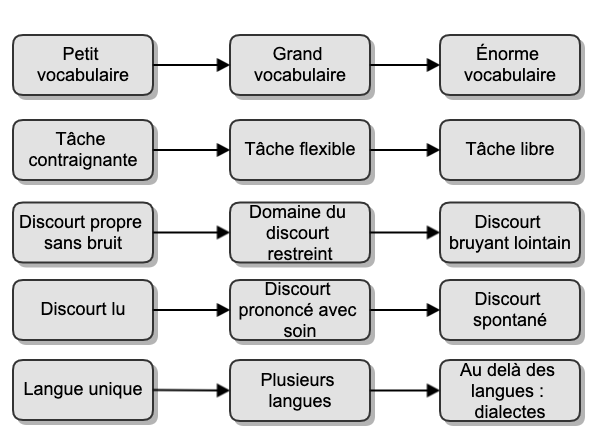
\includegraphics[height=200pt,width=300pt]{images/chap1/evolution_asr.png}
    \caption{Évolution des contraintes lors de la reconnaissance de la parole}
    \label{evolotion}
\end{figure}

\subsection{Utilisation des systèmes de reconnaissance de la parole}
Le fait que la reconnaissance de la parole ait suscité autant d'intérêt ces dernières décennies n'est pas dû au hasard. En effet, ces systèmes sont d'une grande utilité tant pour améliorer la communication entre les humains que la communication entre l'humain et la machine \cite{deeplearningapproach}.

Les systèmes de reconnaissance de la parole peuvent être utilisés, entre autres applications, afin de : 
\begin{itemize}
    \item développer des assistants intelligents basés sur la reconnaissance de la parole qui, de nos jours, sont présents dans beaucoup d'appareils électroniques permettant ainsi à l'utilisateur d'exprimer des requêtes en langage naturel sans avoir à passer par un clavier réduisant ainsi considérablement le temps et les efforts fournis par ce dernier,
    \item faciliter la traduction lors d'une communication orale où les communiquants ne partagent pas la même langue,
     \item gagner en mobilité dans des environnements où une interaction écrite avec nos machines n'est pas possible tel que des travaux manuels ou tout simplement dans sa voiture,
    \item nouveau moyen d'interaction pour les personnes mal voyantes leur permettant ainsi d'interagir avec autrui.
\end{itemize}

\subsection{Architecture d'un système de reconnaissance de la parole basée reconnaissance de phonèmes} \label{Archi1}
Les systèmes basés reconnaissance de phonèmes partagent une architecture commune et ce, indépendamment de la langue traitée. Cette architecture comporte quatre modules principaux qui sont représentés à travers le diagramme suivant \cite{deeplearningapproach} :
\begin{figure}[H]
    \centering
    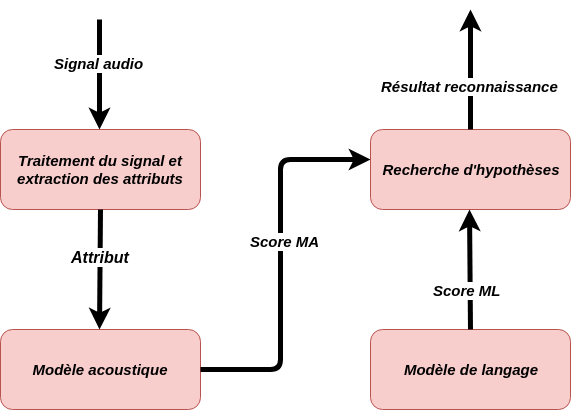
\includegraphics[height=200pt,width=300pt]{images/chap1/architecture_asr.png}
    \caption{Architecture d'un système de reconnaissance de la parole basée reconnaissance de phonèmes}
\end{figure}

Nous présentons dans ce qui suit chaque module de l'architecture :

\subsubsection{Traitement du signal et extraction des attributs}
Traduit de "signal processing and feature extraction", ce module de l'architecture prend un signal audio en entrée, passe par une étape de réduction du bruit suivie de la transformation du signal analogique en fréquences et donne en sortie des vecteurs contenant les caractéristiques de ces fréquences sous forme d'attributs. L'une des méthodes les plus répandues pour l'extraction de ces attributs est l'utilisation du MFCC\footnote{MFCC : Mel Frequency Ceptral Coefficients.} \cite{mfcc} qui prend un enregistrement audio en entrée, y applique un certain nombre de filtres et renvoie en sortie une matrice numérique de caractéristiques qui est un spectrogramme représentant la variation du signal. Nous présentons le MFCC en détail dans le troisième chapitre de ce mémoire.

\subsubsection{Modèle acoustique}
Le modèle acoustique représente la pierre angulaire de cette architecture, il a pour objectif de transformer les informations contenues dans le vecteur de caractéristiques produit par le module précédent (traitement du signal) en unités linguistiques qui seront traitées au niveau du module suivant. \cite{featureextract} présente les approches utilisées pour répondre à ce besoin :
\begin{itemize}
    \item l'approche appelée algorithmes dynamiques de déformation temporelle \cite{terministicapproach} qui a pour but de comparer directement les séquences des données temporelles, tel que des enregistrements audio, en utilisant différentes mesures de distance tel que la distance euclidienne par exemple. Ces approches sont anciennes et très rarement utilisée de nos jours.
    \item l'approche statistique: nous parlons ici de HMM\footnote{Modèles de Markov Cachés, traduit de l'anglais : "Hidden Markov Models"} \cite{hmmtuto} et de GMM\footnote{Modèles de mélange Gaussien, traduit de l'anglais : "Gaussian Mixture Models"} \cite{gmmrobust} mais aussi de modèles d'apprentissage profond ou encore des modèles hybrides HMM-DNN\footnote{Réseaux de Neurones Profonds, traduit de l'anglais "Deep Neural Networks"} \cite{dnnnew}. Ces techniques seront brièvement présentées dans le chapitre 2.	 
\end{itemize}

\subsubsection{Modèle de langage}
Les modèles de langage sont utilisés dans les systèmes de reconnaissance de la parole pour améliorer leur performance. En pratique, ce modèle est utilisé pour rechercher une interprétation de l'entrée du modèle acoustique et prédire une suite de mots correspondant à cette entrée. D'après \cite{languagemodel}, ce modèle peut être basé sur :
\begin{itemize}
    \item une grammaire : Utilisée généralement lorsque la gamme de phrases à reconnaître est restreinte en terme de taille et peut être capturée par une grammaire déterministe. Ce type de modèles est très peu utilisé de nos jours; ou 
    \item un modèle probabiliste, le plus souvent utilisant la notion de N-Grammes \cite{ngramspeech} qui sera détaillée par la suite.\\
\end{itemize}

Le plus grand avantage du modèle de langage est de réduire la perplexité de la reconnaissance en imposant au système de respecter une cohérence dans la suite des mots reconnue par le modèle acoustique et ainsi,  améliorer les performances de la tâche de reconnaissance \cite{langmodelbenefit}.


\subsubsection{Recherche d'hypothèses}
Pour le modèle acoustique et le modèle de langage, un score est généré pour chacun afin d'évaluer le résultat et ce sont ces scores qui sont utilisés dans le module de recherche d'hypothèses.
Ce module compare le score associé au modèle acoustique à celui généré par le modèle de langage afin de décider du résultat final de la reconnaissance. Si le score du modèle de langage est supérieur à celui du modèle acoustique, le système effectue une rectification dans l'ordre d'apparition des mots reconnus  \cite{deeplearningapproach}.
Dans le cas de la reconnaissance de la parole, le score engendré est la performance du modèle qui est représentée par des métriques que nous détaillons dans le chapitre suivant.

La figure \ref{explASRpho} est un exemple de reconnaissance de la parole basée reconnaissance de phonèmes.

\begin{figure}[H]
    \centering
    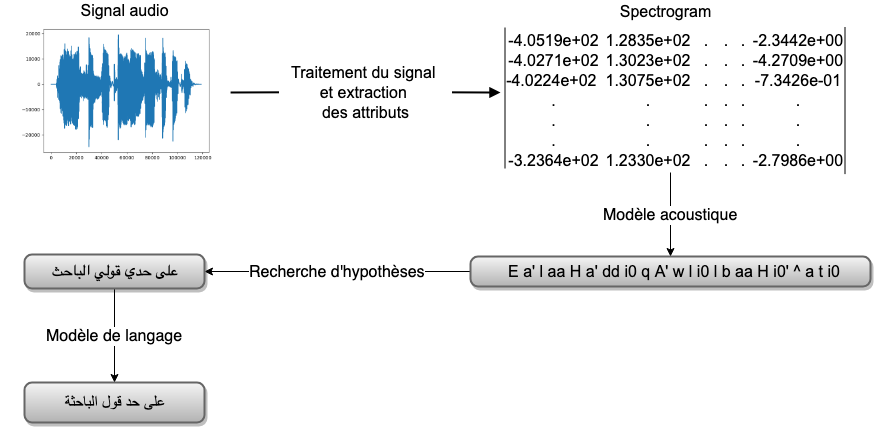
\includegraphics[width=400pt]{images/chap1/Exemple_ASR_Phoneme.png}
    \caption{Exemple de reconnaissance de la parole basée reconnaissance de phonèmes}
    \label{explASRpho}
\end{figure}


\subsection{Architecture End-To-End d'un système de reconnaissance de la parole} \label{Archi2}
L'architecture bout à bout, ou End-To-End en anglais, porte ce nom car contrairement à l'architecture précédente elle consiste en un seul module qui prend en entrée un enregistrement audio et produit la transcription qui y correspond. 
Cette approche pour appréhender les systèmes de reconnaissance de parole a été introduite par \cite{towardse2esr} pour palier aux difficultés rencontrées dans l'approche basée reconnaissance de phonèmes :
\begin{itemize}
    \item complexité de développement
    \item pauvreté des corpus disponibles, et 
    \item barrière de la langue. 
\end{itemize}

Nous commençons par présenter la figure suivante qui illustre les composantes principales de cette architecture : 
\begin{figure}[H]
    \centering
    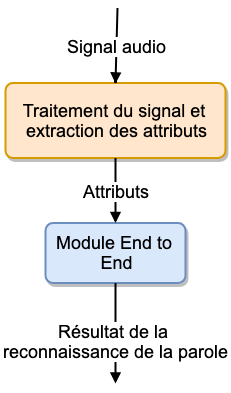
\includegraphics[width=140pt]{images/chap1/E2E_Archi.png}
    \caption{Architecture End-To-End d'un système de reconnaissance de la parole}
\end{figure}

Comme nous le voyons, cette architecture se compose de deux modules principaux.

\subsubsection{Traitement du signal et extraction des attributs}
Ce module a la même fonction que le module portant le même nom dans l'approche basée reconnaissance de phonèmes qui est de générer, à partir d'une enregistrement audio, un spectrogramme sous forme de matrice numérique représentant les variations du signal de l'enregistrement.

\subsubsection{Module End-To-End}
Ce module, que nous considérons pour l'instant comme une boîte noire, est le module qui apprend à générer une transcription à partir d'un spectrogramme jouant ainsi le rôle du modèle acoustique et du modèle de langage. Ce module a donc pour but d'abstraire la difficulté de la tâche de reconnaissance et simplifier le pipeline du développement et ce, en se basant sur des techniques plus récentes d'apprentissage automatique et d'apprentissage profond tel que les réseaux de neurones que nous présentons à travers les deux chapitres suivants.

La figure suivante est un exemple qui a pour but de présenter les étapes de la reconnaissance d'un enregistrement audio pour l'approche End-To-End.

\begin{figure}[H]
    \centering
    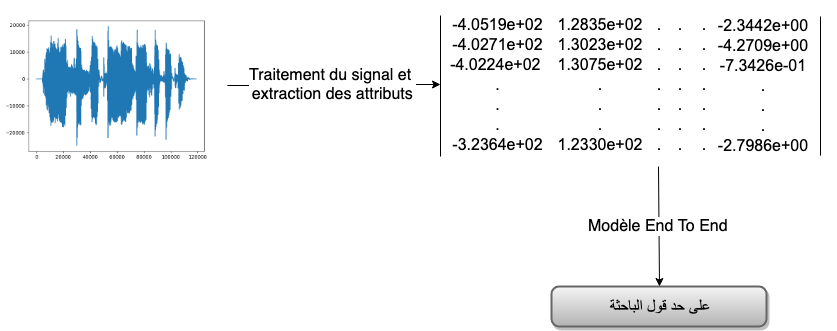
\includegraphics[width=400pt]{images/chap1/Exemple_archi_end2end.png}
    \caption{Exemple de reconnaissance avec l'architecture End-To-End}
    \label{explASRE2E}
\end{figure}


\section{Systèmes de synthèse vocale}
\subsection{Présentation}
Les systèmes de synthèse vocale ou, Text-To-Speech en anglais, sont utilisés pour convertir des mots écrits (dans un document par exemple) en discours audible et doivent êtres capables de lire n'importe quel texte.
Ces systèmes sont largement utilisés de nos jours et il y a de plus en plus d'applications qui fournissant des services de synthèse vocale. L'engouement pour ces systèmes est dû aux possibilités que ceux-ci offrent \cite{ttsuse}, parmis ces possibilités nous citons : 
\begin{itemize}
    \item l'aide aux mal-voyants,
    \item l'aide à l'assimilation des connaissances, 
    \item l'aide à la traduction et à la prononciation, et
    \item les assistants intelligents. \\
\end{itemize}

Comme pour la tâche de reconnaissance de la parole, il existe une approche qui se base sur la synthèse des phonèmes et une approche bout à bout. Nous présentons dans ce qui suit ces deux approches en mettant l'accent sur la complexité de conception d'un système basée synthèse de phonèmes par rapport à un système bout à bout.

\subsection{Architecture d'un système de synthèse vocale basée synthèse de phonèmes}
Les systèmes basés synthèse de phonèmes se basent sur deux parties principales: conversion du texte en phonèmes puis, conversion des caractéristiques linguistiques des phonèmes en discours \cite{textspeechpres}. Nous présentons dans ce qui suit quelques généralités sur cette approche.
Un système de synthèse vocale, indépendamment du texte et de la langue , se compose des modules de base suivants \cite{textspeechmodules} :
\begin{itemize}
    \item \textbf{Conversion de graphème vers phonèmes} : Permet de convertir un texte écrit en phonèmes et ce en utilisant un alphabet phonétique qui est un ensemble de symboles ou de codes utilisés pour indiquer le son d'une lettre (comme Arpabet \cite{arpabet} par exemple).
    \item \textbf{Modèle de segmentation} : il localise les temps de début et fin de chaque phonème et permet d'effectuer un alignement entre les phonèmes ainsi que les lettres présentes présentes dans le catalogue de voix disponible.
    \item \textbf{Modèle de fréquence fondamentale} :  il prédit si un phonème est exprimé et si tel est le cas, il retourne la fréquence du signal correspondante à ce phonème selon la durée de ce dernier.
    \item \textbf{Modèle de synthèse audio} : il combine les sorties des modèles précédents et renvoie en sortie une synthèse vocale du texte désiré. 
\end{itemize}
 
\subsection{Architecture End-To-End d'un système de synthèse vocale}
L'architecture bout à bout \cite{e2espeechsynth} se compose de deux modules principaux comme le montre la figure \ref{E2Esynthese} : 
\begin{figure}[H]
    \centering
    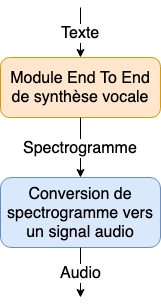
\includegraphics[width=120pt]{images/chap1/Synthese_E2E_Archi.png}
    \caption{Architecture End-To-End d'un système de synthèse vocale}
    \label{E2Esynthese}
\end{figure}

Cette architecture est donc composée des : 

\begin{itemize}
    \item \textbf{Module End-To-End de synthése vocale} : qui prend un texte en entrée et génère à partir de ce texte un spectrogramme. Nous pouvons considérer ce processus comme le processus inverse que celui présenté dans le module séquence à séquence pour les systèmes de reconnaissance de la parole.
    \item \textbf{Conversion de spectrogramme vers signal audio} : ce module permet de convertir un spectrogramme en un signal audio générant ainsi un enregistrement. \\
\end{itemize}

La figure \ref{exempleSyntheseVoc} est un exemple de traduction d'un texte vers un enregistrement sonore à l'aide de l'architecture End-To-End.

\begin{figure}[H]
    \centering
    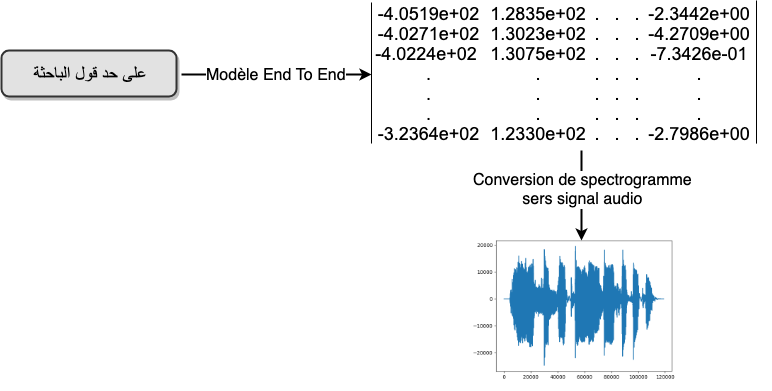
\includegraphics[width=400pt]{images/chap1/Exemple_Synthese_E2E.png}
    \caption{Exemple de synthèse vocale avec l'architecture End-To-End}
    \label{exempleSyntheseVoc}
\end{figure}
\subsection{Quelques applications de synthèse vocale}
Il existe à ce jour plusieurs applications de synthèse vocale \cite{ttsapps}; nous présentons dans ce qui suit les meilleures applications en terme de performance et de simplicité d'utilisation.
\begin{itemize}
    \item \textbf{Amazon Polly} : Alexa n'est pas le seul outil d'intelligence artificielle créé par le géant de la technologie Amazon; il propose également un système de synthèse vocale intelligent appelé Polly \cite{polly} et utilise des techniques avancées d'apprentissage profond. Ce logiciel transforme le texte en discours réaliste et les développeurs peuvent utiliser le logiciel pour créer des produits et des applications embarquant des systèmes de traitement de la parole. Amazon Polly comporte une API permettant d'intégrer facilement les fonctionnalités de synthèse vocale dans des livres électroniques, des articles et d'autres supports. Pour convertir du texte en parole, il suffit de l'envoyer par l'intermédiaire de l'API, qui enverra un flux audio directement à votre application. Amazon Polly est disponible pour plusieurs langues dont l'anglais, le français, le portugais, le japonais et le mandarin. \\
    
    \item \textbf{Voice Reader Home} : basée en Allemagne, Linguatec est une autre société qui crée des applications de synthèse vocale depuis plusieurs années. À présent dans sa 15ème édition, Voice Reader \cite{voicereader} peut convertir rapidement du texte en fichiers audio et peut convertir rapidement des textes tels que des documents Word, des courriels, des EPUB et des PDF pour les écouter sur un PC ou un appareil mobile par la suite. Cette application a l'avantage d'offrir 67 voix différentes et prendre en charge jusqu'à 45 langues telles que l'anglais, l'arabe, le français, l'espagnol, l'italien, le danois et le turc. \\ 
    
    \item \textbf{Capti Voice} : Les applications de synthèse vocale sont également populaires dans le monde de l'éducation, où elles sont notamment utilisées pour améliorer la compréhension. Positionnée comme une solution d'aide à la lecture hors ligne et en ligne, Capti Voice dans sa version 2.0 \cite{captivoice} est utilisée par un grand nombre d'écoles, de collèges, d'entreprises et de professionnels du monde entier. Soutenant plus de 20 langues, dont la langue arabe, l'application peut être utilisée pour améliorer le vocabulaire ainsi que dans le cadre de stratégies de lecture active. Elle peut décrire un éventail de contenus, notamment des livres électroniques, des articles et des pages web. Capti Voice a cependant le désavantage de proposer des licences chères ce qui rend son utilisation très contraignante dans les milieux démunis. \\
    
    \item \textbf{Natural Reader} : c'est une application de synthèse vocale basée sur le cloud et destinée d'avantage à un usage personnel. Natural Reader \cite{naturalreader} permet de convertir des textes écrits tels que des documents Word et PDF, des livres électroniques et des pages Web en des discours continus. Etant basée sur la technologie du cloud, cette application peut accéder au service de synthèse vocale quel que soit le support du moment que l'application est connectée au même service cloud. Natural Reader propose le service de synthèse vocale pour plusieurs langues dont : l'anglais, l'arabe, l'allemand, le français et le mandarin.
\end{itemize}

\subsection{Discussion}
À travers cette présentation, nous notons que le développement d'un système basé synthèse de phonèmes peut s'avérer plus complexe car il nécessite en premier lieu la collecte d'un corpus de données contenant une description des temps de début et de fin de chaque phonème et la collecte d'un tel corpus peut s'avérer délicate comparée à la collecte d'un simple corpus d'enregistrements sonores et transcriptions pour l'approche End-To-End. En plus de cela, l'approche End-To-End présente un développement plus intuitif et plus prometteur grâce à l'avancée des technologies qui y sont utilisées. 

Nous nous contentons de ces généralités en ce qui concerne les architectures des systèmes de synthèse vocale car le corps de notre travail consiste à développer un système de reconnaissance de la parole et son application sur une problématique donnée. Nous introduisons dans ce qui suit les systèmes de questions-réponses, leurs différents types ainsi qu'une présentation de quelques exemples de ces systèmes.

\section{Les systèmes de questions-réponses}
\subsection{Présentation}
Les systèmes de questions-réponses sont des systèmes intelligents. Selon  \newline \cite{QAS}, un système de questions-réponses est un système d'information capable de comprendre des questions et y répondre de manière précise dans un langage naturel humain comme par exemple donner une réponse à la question "Quels sont les meilleurs laboratoires de recherche en intelligence artificielle ?"

Les systèmes de questions-réponses sont généralement classifiés selon le domaine auquel ils appartiennent ainsi que le type de questions.

\subsection{Classification des systèmes de questions-réponses par domaine} \label{QASdomain}
Nous commençons par introduire les deux domaines auxquels peuvent appartenir les systèmes de questions-réponses. D'après \cite{Types_QAS_Survey} ceux-ci peuvent être ouverts ou fermés.
\subsubsection{Domaine ouvert}
Les systèmes de questions-réponses de domaine ouvert sont des systèmes qui ne sont pas limités à un domaine spécifique. En d'autres termes, pour cette classe de systèmes, l'utilisateur a la possibilité d'introduire la question qu'il désire dans le système étant donné que ce type de systèmes recherche généralement les réponses dans une grande collection de documents comme les recherches sur le web à titre d'exemple.

\subsubsection{Domaine fermé}
Les systèmes de questions-réponses appartenant au domaine fermé consistent en un référentiel limité de questions spécifiques à un domaine (le domaine médical à titre d'exemple) et peuvent répondre à un nombre limité de questions. La qualité des réponses dans le domaine fermé est élevée, les réponses sont obtenues à partir de données structurées (telles que des bases de données), des données semi-structurées (par exemple, des textes annotés au format XML) ou des données non structurées (textes libres).
% ici classification des SQR par type de question
\subsection{Classification des systèmes de questions-réponses par types de questions} \label{QASqstType} 
Le type de la question posée par un utilisateur est très important car il permet de déduire, à priori, le type de réponse attendue et ainsi de générer cette dernière d'une manière plus efficace. 
Les différents types de questions posées par les utilisateurs sont classés d'après \cite{qstClassif} en :
\begin{itemize}
    \item questions de type factoïde, 
    \item questions de type liste,
    \item questions de confirmation, et 
    \item questions de causalité.\\
\end{itemize}

Prenons pour exemple la question "Qui était le premier président de l'Algérie?", le domaine de la question posée par l'utilisateur est l'histoire de l'Algérie, la réponse attendue est une entité nommée et plus précisément le nom d'une personne qui est “Ahmed Benbella”. Cette question est de type factoïde.

Dans le tableau \ref{table:qstclass} nous présentons les principaux types de questions.

\FloatBarrier
\begin{center}
    \begin{table}[h]
    \caption{Classification des questions par type  de réponse}
    \label{table:qstclass}
    \begin{tabular}{|c|c|c|}
        \hline
         \thead{Type} & \thead{Réponse attendue} & \thead{Exemple}\\
         \hline
         \makecell[l]{Factoïde} & \makecell[l]{Entité nommée (nom d'une \\ personne nom d'une organisation, \\lieu ou date)} &  \makecell[l]{\textbf{Question} : Quelle est\\la capitale de l'Algérie ?\\ \textbf{Réponse} : Alger.} \\
         \hline
         \makecell[l]{Liste} & \makecell[l]{Une liste d'entités nommées} & \makecell[l]{\textbf{Question} : quels sont les\\ pays les plus propres\\ du monde?\\ \textbf{Réponse} : Suède, Nouvelle\\ Zélande, Australie, \\Canada.}\\
        \hline
        \makecell[l]{Définition}  & \makecell[l]{Information concernant\\ une entité nommée} & \makecell[l]{\textbf{Question} : Qui est \\Thomas Pesquet ?\\\textbf{Réponse} : un spationaute\\français de l'Agence\\spatiale européenne.}\\
        \hline
        \makecell[l]{Confirmation} & \makecell[l]{Les réponses peuvent être de \\ différents types : \\ Oui/Non Arguments, etc.} & \makecell[l]{\textbf{Question} : Est-ce-que\\l'USTHB se situe en Algérie \\ \textbf{Réponse} : Oui.} \\
        \hline
        \makecell[l]{Causale} & \makecell[l]{Des explications sur une entité.} & \makecell[l]{\textbf{Question} : Pourquoi les \\abeilles  produisent du miel? \\ \textbf{Réponse} : Les abeilles \\ fabriquent  du miel pour \\ nourrir les larves  et surtout\\ pour avoir des  réserves de \\nourriture en hiver.}\\
        \hline
    \end{tabular}
    \end{table}
\end{center}
\FloatBarrier

\subsection{Architecture des systèmes de questions-réponses}
L'architecture type d'un système de questions-réponses (voir la figure \ref{ArchiQAS}) se compose de trois modules principaux \cite{thesisasma} : un module d'analyse des questions, un module de traitement des documents et un module d'extraction et validation de la réponse.

\subsubsection{Module d'analyse des questions}
Dans ce module, la question posée par l'utilisateur est analysée afin d'identifier son type, d'en extraire les caractéristiques et la structure de la réponse attendue et de déterminer les contraintes qui pèsent sur la réponse attendue.
\subsubsection{Module de traitement des documents}
Ce module est un composant essentiel du système de questions-réponses. Son rôle est d'extraire les documents et les passages pertinents pour la question à partir d'une collection de données (Web ou autre) pour effectuer ensuite un processus de classement qui permettra d'améliorer la pertinence des passages candidats qui correspondent le mieux à la question de l'utilisateur.
\subsubsection{Module d'extraction et validation de la réponse}  
Dans les systèmes de questions-réponses, ce module peut être conçu pour extraire la réponse à partir d'un ou plusieurs passages. Ce module ne renvoie la réponse que si les passages candidats fournis par le module de traitement des documents sont pertinents et contiennent réellement la réponse. Certains systèmes intègrent également la validation des réponses dans ce module. 
\begin{figure}[H]
    \centering
    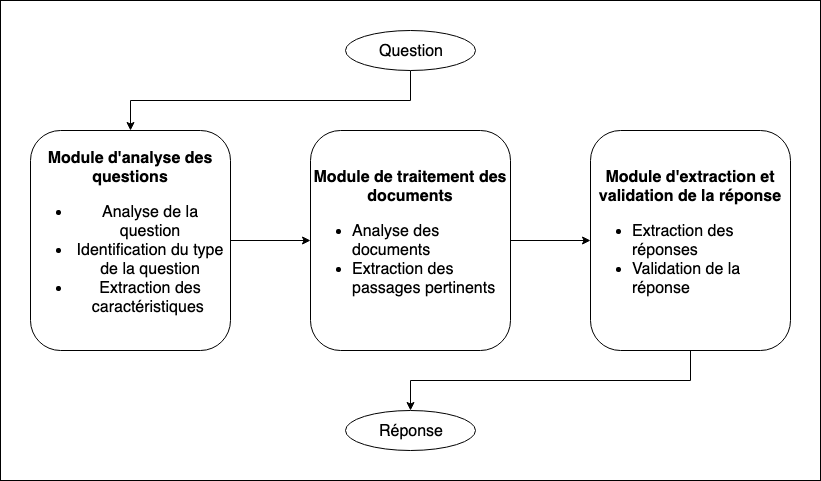
\includegraphics[height=200pt,width=325pt]{images/chap1/QAS_archi.png}
    \caption{Architecture générique d'un système de questions-réponses}
    \label{ArchiQAS}
\end{figure}


\subsection{Quelques systèmes de questions-réponses}
Les systèmes de questions-réponses pour la langue arabe ne sont pas aussi nombreux que pour l'anglais par exemple, ce qui peut s'expliquer par le nombre limité de corpus de qualité existants.

Dans ce qui suit, nous présentons quelques exemples de systèmes de questions-réponses pour la langue anglaise et la langue arabe.


\subsubsection{Start}
START est un des systèmes de questions-réponses les plus connus pour la langue anglaise. Développé par Boris Katz et ses collaborateurs du groupe InfoLab du laboratoire d'informatique et d'intelligence artificielle du MIT, START est en ligne depuis 1993 \cite{StartPaper}. Actuellement, ce système peut répondre à des millions de questions en anglais en langage naturel. Les réponses sont en format texte ou multimédia qui sont tirés d'un ensemble de ressources d'informations hébergées localement ou accessibles à distance via Internet.

% START vise une grande précision dans la réponse à ses questions et, en grande partie, sa capacité à répondre aux questions se fait grâce à l'utilisation des annotations en langage naturel en tant que mécanisme d'ajustement des questions aux réponses des candidats. 

% Lorsque de nouvelles ressources d'information sont incorporées pour l'utilisation de START, les annotations en langage naturel sont souvent composées manuellement - généralement à un niveau abstrait - puis associées à divers composants d'information. Bien que l'effort START ait également exploré diverses techniques pour la génération automatique d'annotations, le présent document porte sur l'utilisation des annotations composées manuellement dans START et ses systèmes affiliés, ainsi que sur les avantages qui en découlent.

% \subsection{Travaux sur la langue arabe}
% L'arabe est la 6ème langue naturelle la plus répandue au monde avec plus de 350 millions de locuteurs natifs. Les systèmes de questions-réponses en arabe gagnent en importance en raison de la quantité croissante du contenu en arabe et de la demande croissante d'informations que les techniques habituelles de recherche d'information ne peuvent satisfaire.
% Malgré cela, ces systèmes rencontrent des difficultés en terme de ressources. Comparé à d'autres langues, les corpus utilisés sont peu volumineux et manquent en diversité du contenu. Dans ce qui suit nous présentons les systèmes que nous jugeons être les plus intéressants en la matière.

\subsubsection{DefArabicQA}
DefArabicQA \cite{ArabicQA}  est un système de questions-réponses de définition, en d'autres termes ce système traite les questions du type \setcode{utf8}\<ما هو ؟> ou \setcode{utf8}\<ما هي ؟> . Il identifie les définitions candidates en utilisant un ensemble de modèles lexicaux \footnote{Un modèle lexical est une séquence de chaînes de caractères (par exemple, des mots, des lettres et des signes de ponctuation) qui fournissent un contexte pour identifier les réponses exactes \cite{ArabicQA}.}, filtre ces définitions candidates en utilisant des règles heuristiques qui se déduisent de l'observation d'un ensemble de définitions candidates annotées\footnote{Un ensemble de définitions candidates divisées en définitions de candidats incorrectes et correctes} et les hiérarchise en utilisant une approche statistique. Le type de réponse attendu est déduit par la suite du pronom interrogatif de la question.
% Dans \cite{ArabicQA}, Trigui1 et al. ont effectué deux expériences d'évaluation sur 50 questions de définition. 
% \begin{center}
%     \begin{table}[H]
%         \centering
%         \begin{tabular}{|c|c|c|}
%             \hline
%             \thead{Expérience} & \thead{ressource Web} & \thead{MRR}\\
%             \hline
%             \makecell{1} & \makecell{Google} & \makecell{0,70}  \\
%             \hline
%             \makecell{2} & \makecell{Google couplé \\ à Wikipédia} & \makecell{0,81}  \\
%             \hline
%         \end{tabular}
%         \caption{Expériences d'évaluation de DefArabicQA}
%         \label{tab:my_label}
%     \end{table}
% \end{center}

\subsubsection{Al-Bayan}
Al-Bayan \cite{Albayan} est un système de questions-réponses spécifique au Coran. Il prend une question en arabe en entrée et récupère des versets  accompagnés de leur \textit{tafsir} (interprétation des versets) sémantiquement pertinents en tant que passages candidats.

La spécificité de ce système réside dans le fait qu'il automatise le processus de sélection des réponses. Les réponses candidates sont ensuite classées en :
\begin{itemize}
    \item Réponses qui répondent directement à la question.
    \item Réponses qui peuvent être utiles.
    \item Réponses qui ne sont pas pertinentes.
\end{itemize}


\section{Conclusion}
Au vu de l'importance des systèmes de reconnaissance de la parole, l'étude de ces derniers et leur implémentation pour la langue arabe dans des applications telles que les systèmes de questions-réponses est devenu un besoin pour le monde arabe en particulier et pour les utilisateurs de l'arabe de manière générale. Au cours de ce chapitre, nous avons abordé les aspects de bases des systèmes de reconnaissance de la parole, systèmes de synthèse vocale ainsi que des systèmes de questions-réponses comme cas d'application pour la reconnaissance de la parole.

Dans le chapitre suivant, nous introduisons les différentes approches utilisées pour le développement d'un système de reconnaissance de la parole pour ensuite présenter les travaux faisant état de l'art tant pour la langue arabe que pour les autres langues afin de nous guider à concevoir notre propre système.

    


%%% References %%%
\newpage
\pagenumbering{gobble} 
\bibliographystyle{unsrt} 
\bibliography{ref}

\end{document}
%~~~END~~~%
